\documentclass[11pt]{article}
\usepackage{geometry}                % See geometry.pdf to learn the layout options. There are lots.
\usepackage{graphicx}
\usepackage{amssymb}
\usepackage{epstopdf}
\DeclareGraphicsRule{.tif}{png}{.png}{`convert #1 `dirname #1`/`basename #1 .tif`.png}

\textwidth6.5in
\textheight9.0in
\topmargin-0.5in
\oddsidemargin0in
\evensidemargin0in

\title{Implementation of Crack and Material Velocity Fields with Contact and Nodal Velocity Boundary Conditions}
\author{John Nairn}
\date{\today} 

\font\tenbsf=cmssbx10 at 11pt
\font\bfsym=cmmib10 at 11pt



\begin{document}
\maketitle

\section{Velocity Fields}

Each node has one to four crack velocity fields denoted [0], [1], [2], and [3]. If the problem has no cracks, then each node has just the single crack velocity field [0]. Each crack velocity field has any number of material velocity fields or just one velocity field if using single material mode.

\subsection{Crack Velocity Fields}

The crack velocity field is determined by drawing a line from the particle to the node. If the line crosses no cracks, that material point uses field [0]. If the line crosses one crack, that material point uses field [1] (for the first crack found) or field [2] (if a second crack is found for the same node). If the line crosses two cracks, the material point uses field [3]. This scheme can handle one or two cracks at each node. A third crack ({\em i.e.}, a line that crosses a third crack or one of the cracks in field [3] being different than the cracks for fields [1] and [2]) is handled by picking one of the four fields, but is likely to not get the physics correct. A warning is issued if a third crack is found.

Figure \ref{cvf}\ shows schematic view of crack velocity fields for the indicated nodal point. Because field [2] is never allocated before field [1] ({\em i.e.}, the first single crack crossing is put into field [1] and the second into field [2]), the following crack field situations are all that are possible: [0], [1], [3], [0]\&[1], [0]\&[3], [1]\&[2], [1]\&[3], [0]\&[1]\&[2], [0]\&[1]\&[3], [1]\&[2]\&[3], and [0]\&[1]\&[2]\&[3]. The combinations that never occur are the remaining ones or [2], [0]\&[2], [2]\&[3], and [0]\&[2]\&[3].

When doing crack contact, the possible field contacts are between [0]\&[1] and [2]\&[3] on the crack \#1 surface and between [0]\&[2] and [1]\&[3] on the crack \#2 surface. Fields [0]\&[3] and [1]\&[2] do not contact each other.

\begin{figure}
\begin{center}
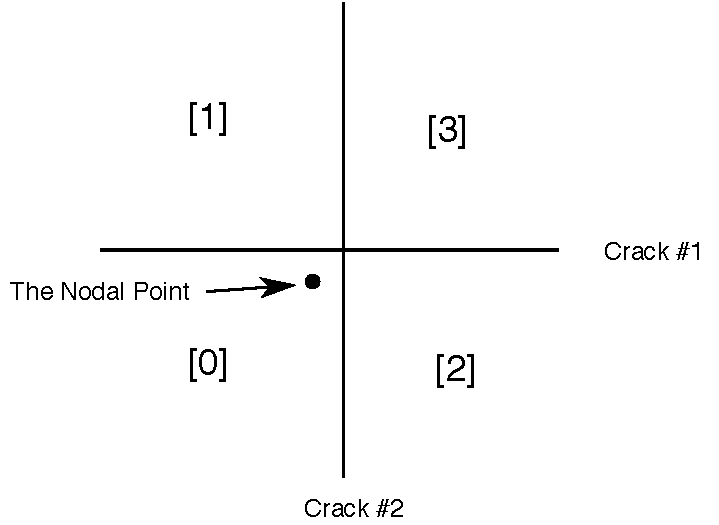
\includegraphics{CrackFields}
\caption{Schematic view of crack velocity fields around a single node. The possibility of two interacting cracks leads to at most four velocity fields.}
\label{cvf}
\end{center}
\end{figure}

\subsection{Material Velocity Fields}

Each crack velocity field may have 1 to $n$ material velocity fields where $n$ is the number of materials assigned to material points. For a single velocity field, $n$ is set to 1 and all materials use the same velocity field.

\section{MPM Time Step Tasks}

This section lists each task in NairnMPM outlining only those parts relevant to crack and material velocity fields, to contact conditions, to imperfect interface and traction laws on cracks, and to nodal velocity boundary conditions.

\subsection{Task 0: Initialization}

Each nodal point is permanently assigned field [0] and that field is zeroed. Any material velocity fields in field [0] that were used in the last step are also zeroed. If the previous step allocated fields [1], [2], or [3], they are deleted. 

For each material point, find the crack velocity field (${\tt vfld}=0,\ 1,\ 2$, or $3$) by checking the line crossings of all cracks (if there are no cracks {\tt vfld} is always 0). This task was moved to initialization when code went parallel. It is one of the largest tasks that is not parallelized.

\subsection{Task 1: Project Momentum and Mass to the Grid}

For each material point, look for the crack velocity field and determine the appropriate material field ({\tt matfld}) from the material assigned to that material point. Add the momentum and mass to material velocity field {\tt matfld} of crack velocity field {\tt vfld} . For crack contact and imperfect interface calculations, project the displacement (or position) and undeformed volume for crack velocity field {\tt vfld} to the grid. This displacement and undeformed volume treats all materials in the crack velocity field as a single material velocity field.

\subsection{Task 2: Contact and Optional Update Strains First}

Adjust momenta at all overlapping material velocity fields in each crack velocity field using the material-material contact law. Next adjust momenta for crack contact conditions. The crack contact calculations use the center-of-mass material velocity field for that crack velocity field. Then, for each node with a fixed velocity on any component of velocity, copy all velocity fields (these are denoted as $p_{int}$ or the initially interpolated velocity and will will be needed in task 3) and then set the corresponding component to the prescribed momentum.

Note: I used to prescribe boundary conditions before doing contact, but now do the contact calculations first. The logic being that the projected velocity fields before prescribing boundary conditions for multiple velocity fields with cracks in which contact is done by stick conditions should be identical to those for a single velocity field/no-crack calculation. Doing contact before boundary conditions achieves this goal.

When updating strains first (or first and last), calculate velocities in all velocity fields and update the strains and stresses.

\subsection{Task 3: Project Forces to the Grid}

For each material point, project $f_{int}$ and $f_{ext}$ to the grid. These are added to material velocity field {\tt matfld} of crack velocity field {\tt vfld}, where {\tt vfld} was found in task  and {\tt matfld} is known by the material point's material type.

For all cracks with traction laws, add $f_{ext}$ for the traction. For all cracks with imperfect interfaces, add $f_{int}$ due to interfacial displacements (note: it might be possible to do material contact by an interface law as well).

Finally, revisit all nodes with velocity boundary condition and change to total force to the force required to convert $p_{int}$ to the boundary condition momentum $p_{BC}$ after the task 4 momentum update using the relation:
\begin{equation}
         f_{tot} = {p_{BC}-p_{int}\over \Delta t}
\end{equation}
where $\Delta t$ is the time step. This step is essential to get consistent forces and momenta, which are converted to accelerations and velocities during the particle update in task 5. Moreover, if force or momentum are changed again between this task and the particle update, they {\em must} be changed together to remain consistent.

\subsection{Task 4: Update Nodal Momenta}

This task updates the nodal momenta using
\begin{equation}
     \vec p_{k+1} = \vec p_k + f_{tot}\Delta t
\end{equation}
Now, depending on the problem, this update may cause more contact. Thus the update must be followed by adjusting momenta at all nodes with overlapping materials and at all cracks now in contact. The logic again is that the final momenta in this step should be identical when doing multiple velocity fields with stick contact to the momenta when using a single velocity field.

Two details are important. First, because of the need to keep momenta and forces consistent until the particle update in task 5, any time the momentum is changed by $\Delta\vec p$, the corresponding force must be changed by $\Delta\vec p/\Delta t$.

Second, the momentum component for any node that fixes that component with a velocity boundary condition must not be changed. If boundary conditions are applied to all velocity fields, this situation may never arise because the boundary conditions should insure the momentum update does not induce new contact ({\em i.e.}, the velocity fields will be moving at the same velocity).


\subsection{Task 5: Update the Particles}

Update particle position and velocity using nodal velocity (from momentum) and acceleration (from $f_{tot}$) found in material velocity field {\tt matfld} of crack velocity field {\tt vfld}.

\subsection{Task 6: Optional Update Strain Last}

My reading of the Sulsky, Zhou, Scherer paper that claimed to improve the original Sulsky paper by dealing with modal momentum rather than nodal velocities, is really that the algorithm projects momenta to the grid a second time prior to updating strains. Thus, this task rezero's all velocity field momenta, loops over particles, and projects to the grid. The projection uses the pre-calculated material velocity field {\tt matfld} of crack velocity field {\tt vfld}. For crack contact calculations, also project the displacements for each crack velocity field. Because this projection might induce new contact, adjust momenta again at nodes with multiple materials and at crack surfaces. Again, the logic is make sure stick conditions are identical to single velocity field and a single velocity field would not permit overlap at this stage.

Finally, impose boundary conditions, calculate nodal velocities (from the final momenta), and update stresses and strains.

\subsection{Task 7: Custom Tasks}

Nothing here is related to contact or to velocity boundary conditions.

\subsection{Task 8: Move Cracks}

The crack surfaces and crack plane are updated using the center-of-mass velocity field of each crack velocity field (for those that have multiple materials).

\section{Contact Forces and Changes in Momentum}

Once contact is detected, the key task is to change the momenta for the various fields to implement stick or frictional sliding. Consider two materials, $a$ and $b$, with nodal velocities on the same node of $\vec v_a$ and $\vec v_b$ and define a normal vector, $\hat n$, that is positive when directed from material $a$ to $b$. The center of mass velocity is
\begin{equation}
     \vec v_c = {m_a \vec v_a + m_b \vec v_b\over m_a + m_b}
\end{equation}
where $m_a$ and $m_b$ are the masses for the two materials. Next, define $\Delta\vec p_a$ as the momentum change required on material $a$ for its velocity to change from $\vec v_a$ to $\vec v_c$ or
\begin{equation}
         \vec v_a + {\Delta\vec p_a\over m_a} = \vec v_c \quad{\rm which\ means}\quad  \Delta \vec p_a = -m_a(\vec v_a -\vec v_c)
\end{equation}
Inserting the definition of $\vec v_c$ leads to
\begin{equation}
       \Delta \vec p_a = -m_a(\vec v_a -\vec v_c) = m_b (\vec v_b -\vec v_c) = {m_a\vec p_b-m_b\vec p_a\over m_a+m_b}
\end{equation}
where $\vec p_a$ and $\vec p_b$ are the nodal momenta for the two materials. Notice that
\begin{equation}
    \Delta \vec v = \vec v_b - \vec v_a = {\Delta \vec p_a\over m_b} + {\Delta \vec p_a\over m_a} = {\Delta\vec p_a\over m_{red}}
\end{equation}
where $m_{red} = m_a m_b/(m_a+m_b)$ is the reduced nodal mass. Thus the relative velocity of approach of the two surfaces is proportional to, and in the same direction as, $\Delta \vec p_a$. However contact is detected, one of the criteria should be that the two surfaces are approaching each other. With the above definition for the one normal, this criteria implies $\Delta\vec v\cdot\hat n<0$ or identically that $\Delta\vec p_a\cdot\hat n<0$. We thus assume that under all contact situations that $\Delta\vec p_a\cdot\hat n<0$.

In simulations with more than two materials, a single node may have velocity fields from three or more materials. This situation may mean contact is not handled well ({\em i.e.}, that resolution needs to be increased until no nodes see three or more materials, if possible) or may mean an unavoidable situation ({\em e.g.}, meeting at corners of materials). The code needs to proceed as well as it can. The approach is to take the center of mass results
\begin{equation}
     \vec p_c = \sum_i \vec p_i  \qquad m_c =  \sum_i m_i \qquad    \vec v_c = {\vec p_c\over m_c}
\end{equation}
and define a {\em virtual} material $b$ derived from all mass and momentum not associated with material $a$:
\begin{equation}
     \vec p_b = \vec p_c-\vec p_a  \qquad m_b = m_c - m_a \qquad    \vec v_b = {\vec p_b\over m_b}
\end{equation}
The equations for $\Delta \vec p_a$ and $\Delta \vec v$ are unchanged, but in terms of just $a$ and $c$, they become
\begin{equation}
    \Delta \vec p_a = {m_a\over m_c}\vec p_c-\vec p_a  \qquad \Delta \vec v = {m_c\over m_a(m_c-m_a)}\Delta \vec p_a
\end{equation}

To implement contact conditions, with inclusion of nodes with three or more materials, each material is considered relative to the center of mass velocity and $\Delta \vec p_a$ and $\Delta \vec v$ are found. Stick conditions are trival. The momentum change of $\Delta \vec p_a$ is applied to material $a$. These momenta changes correspond to normal and tangential forces of
\begin{equation}
         \vec f_n = {(\Delta \vec p_a\cdot \hat n)\over \Delta t}\hat n \qquad {\rm and}\qquad \vec f_t={(\Delta \vec p_a\cdot \hat t)\over \Delta t}\hat t
\end{equation}
where $\Delta t$ is time step and $\hat t$ is unit vector in the tangential direction of motion. We choose $\hat t$ to be in the same direction as the relative motion in the tangential direction such that $(\vec v_b-\vec v_a)\cdot \hat t>0$ and identically such that $\Delta \vec p_a\cdot \hat t>0$ or that the angle between $\hat t$ and $\vec v_b-\vec v_a$ is between -90 and 90 degrees. From the known $\hat n$, the tangential vector is found from
\begin{equation}
          \Delta\vec p_a - (\Delta \vec p_a\cdot \hat n)\hat n = m_{red}(\Delta \vec v\cdot \hat t)\hat t
\end{equation}
The vector on the left can be calculated from prior results and is seen to be parallel to $\hat t$. There are two solutions for $\hat t$ for the two directions along the parallel. We choose the solution such that  $\Delta \vec v\cdot \hat t>0$ or equivalently that $\Delta \vec p_a\cdot \hat t>0$.

The positive normal contact force is thus $f_n = -(\Delta \vec p_a\cdot \hat n)/\Delta t$ and the positive sliding force is $f_t = (\Delta \vec p_a\cdot \hat t)/\Delta t$. If $f_t<\mu f_n+s_a$, the objects will stick using the above stick conditions (here $s_a$ is an optional adhesion strength). Otherwise, the frictional force is changed to $\mu f_n+s_a$, but it still sticks in the normal direction. The complete frictional sliding algorithm in an optimized form is
\begin{enumerate}

\item Determine if contact is occurring. Those calculations will find $\Delta p_a$ and $\hat n$ and will verify that $d_n = \Delta \vec p_a\cdot \hat n<0$. Finding an accurate normal is crucial. The recommended method is to consider the gradient of the volume gradient for the contacting pair of materials (when three or more material are present, the algorithm looks at the volume gradient from material $a$ and the other material with the most volume). The normal is taken as being in the direction of the volume gradient for the material that has the largest magnitude of its volume gradient.

\item Find an unnormalized tangent vector from $\vec t = \Delta p_a - d_n\hat n$. If $\vec t\cdot\vec t=0$, then there is no tangential motion and the momentum change $\Delta p_a$ can be used and the algorithm is done ({\em i.e.}, skip to step 5 with $\Delta \vec {p'}_a =\Delta \vec p_a$). If it is not zero, proceed to next step.

\item Normalize $\hat t$ and find $d_t = \Delta \vec p_a\cdot \hat t$. Since $\hat t$ is defined from the tangential component of $\Delta\vec p_a$, $d_t\ge0$. The zero option is handled in previous step, so now it must be non-zero and positive.

\item If $f_t > \mu f_n+s_a$ (or $d_t>-\mu d_n+s_a\Delta t$), both sides of which are always positive, then frictional sliding is occurring. The force to make material $a$ ``stick'' in normal direction and feel ``frictional'' force in tangential direction is $\vec f_a = (-f_n)\hat n + (\mu f_n+s_a)\hat t$. Thus,  the momentum change for material $a$ becomes $\Delta \vec {p'}_a = \vec f_a\Delta t = d_n(\hat n - \mu\hat t)+s_a\hat t\Delta t $. But, if $d_t<-\mu d_n+s_a\Delta t$, use $\Delta \vec {p'}_a =\Delta \vec p_a$; {\em i.e.}, use the stick-condition momentum change.

\item Change momenta of material $a$ by $\Delta\vec {p'}_a$

\item If the node has only two materials and the method to find normals is the same for both materials, then change momenta of material $b$ by $-\Delta\vec {p'}_a$ and this node is done. If three or more materials are present, or if normals may differ, proceed to next material at this node.

\end {enumerate}

\subsection{Low Mass Situations}

The above algorithm never divides by a possibly low mass, but that does not necessarily mean it is not affected by one of the masses being very low. In GIMP calculations it will be common for a node one element away from the contact region to have nearly all mass in one material and a very low mass in the other material. When that occurs:
\begin{equation}
         {\rm if\ } m_a << m_b, {\rm\ then\ } \Delta \vec p_a \approx m_a\vec v_b -\vec p_a
         \quad {\rm or}\quad
         {\rm if\ } m_b << m_a, {\rm\ then\ } \Delta \vec p_a \approx \vec p_b - m_b \vec v_a
\end{equation}
In other words, $\Delta\vec p_a$ will be based on the unreliable nodal momentum (since it is likely to be from one particle on the edge of a material). Since $\Delta\vec p_a$ is used to determine contact and to adjust the momenta, the entire algorithm will be unreliable. Now, since $\Delta\vec p_a$ will also be very small, it might not make a difference, but in one calculation sliding down an incline plane, the calculation stopped when accepting all contact situations and was fixed by screening out those with $m_a/(m_a+m_n)$ or $m_b/(m_a+m_n)$ less than $10^{-6}$. Thus in step one above, if the mass ratio meets these criteria, ignore contact for that node.

\subsection{Rigid Material Contact}

If material $b$ is rigid, contact can be handled by a special case of the two-material contact, A rigid material corresponds to $m_b\to\infty$. The basic contact equations change to
\begin{eqnarray}
     \vec v_c & = &  \vec v_b \\
     \Delta \vec p_a & = & -m_a(\vec v_a -\vec v_b) \\
     \Delta \vec v & = & \vec v_b - \vec v_a  = {\Delta\vec p_a\over m_a} \\
     m_{red} & = & m_a
\end{eqnarray}
After these changes, the contact methods above can be applied the same way except the momentum of the rigid particle is not changed. In {\tt NairnMPM}, the density of rigid materials is set to 1000 g/cm$^3$ such that material point mass found in {\tt NairnMPM::PreliminaryCalcs()} is equal to the volume for the rigid material point in mm$^3$. Thus the mass gradient needed in the contact algorithm is equal to the volume gradient. The nodal mass, however, for material velocity field of rigid particles is set to zero as a way to determine a rigid particle velocity field. The nodal {\tt vk} is always the correct velocity and is calculated when the first rigid particle is extrapolated to that node.


\end{document}   